\documentclass[11pt,a4paper]{article}
\usepackage[margin=2cm]{geometry}
\usepackage{amsmath,amssymb}
\usepackage{tcolorbox}
\usepackage{booktabs}
\usepackage{enumitem}
\usepackage{hyperref}
\usepackage{xcolor}
\usepackage{fancyhdr}
\usepackage{tikz}
\usetikzlibrary{automata, positioning, arrows.meta}
\usepackage{listings}
\usepackage{adjustbox}

\tcbuselibrary{breakable,skins}

% ── Prevent math overflow in boxes ──────────────────────────────────────────
\newcommand{\fitmath}[1]{\begin{adjustbox}{max width=\linewidth}$\displaystyle #1$\end{adjustbox}}

% ── Listings config ─────────────────────────────────────────────────────────
\lstset{
  basicstyle=\ttfamily\small,
  breaklines=true,
  breakatwhitespace=false,
  breakautoindent=true,
  postbreak=\mbox{\textcolor{gray}{$\hookrightarrow$}\space},
  columns=fullflexible,
  keepspaces=true,
  xleftmargin=0pt,
  xrightmargin=0pt,
  aboveskip=4pt,
  belowskip=4pt,
  frame=none,
  commentstyle=\color{gray},
}

% ── Box definitions ─────────────────────────────────────────────────────────
\newtcolorbox{definitionbox}[1]{colback=blue!5, colframe=blue!60!black,
  fonttitle=\bfseries, title=#1, breakable, enhanced jigsaw}

\newtcolorbox{conceptbox}[1]{colback=red!5, colframe=red!60!black,
  fonttitle=\bfseries, title=#1, breakable, enhanced jigsaw}

\newtcolorbox{examplebox}[1]{colback=green!5, colframe=green!50!black,
  fonttitle=\bfseries, title=#1, breakable, enhanced jigsaw}

\newtcolorbox{notebox}[1]{colback=orange!5, colframe=orange!60!black,
  fonttitle=\bfseries, title=#1, breakable, enhanced jigsaw}

\newcommand{\kemark}{\textcolor{red!70!black}{\textbf{[EXAM-RELEVANT]}}}
\newcommand{\kbg}{\textcolor{gray}{\textbf{[BACKGROUND]}}}
\newcommand{\kt}[1]{\par\vspace{0.3em}\colorbox{yellow!60}{\parbox{\dimexpr\linewidth-2\fboxsep}{#1}}\vspace{0.3em}}

\pagestyle{fancy}
\fancyhf{}
\lhead{AC Lecture 2 --- Cheatsheet}
\rhead{Jawad M.K. Qayyum}
\rfoot{\thepage}

\setlength{\parindent}{0pt}
\setlength{\parskip}{0.4em}

\begin{document}

\begin{center}
{\Huge\bfseries AC Lecture 2}\\[0.5em]
{\LARGE The Church-Turing Thesis}\\[0.3em]
{\large The Complete Guide to ``Why TMs Are Enough'' and ``What Are the Variants?''}\\[1em]
{\normalsize Algorithms and Computability --- Semester 6}\\
{\normalsize Cheatsheet for split-view study with slides}\\[0.5em]
{\normalsize April 2026}
\end{center}

\vspace{1em}
\tableofcontents
\newpage

%═══════════════════════════════════════════════════════════════════════════════
\section{The Big Picture}
%═══════════════════════════════════════════════════════════════════════════════

%───────────────────────────────────────────────────────────────────────────────
\subsection{Where We've Been}

\begin{itemize}[nosep]
\item \textbf{Lecture 1 --- Intro + Turing Machines:}
  \begin{itemize}[nosep]
  \item A \textbf{problem} = a formal \textbf{language} $L \subseteq \Sigma^*$ (a set of strings)
  \item An \textbf{algorithm} = a \textbf{Turing machine} (DTM), defined as $(Q, \Sigma, \Gamma, s, t, r, \delta)$
  \item \textbf{Computable} language = recognized by a \textit{halting} DTM (always stops)
  \item \textbf{Computably-enumerable} language = recognized by some DTM (may loop on non-members)
  \item We built a TM for $\{w\#w \mid w \in \{0,1\}^*\}$ using ``mark, scan, match'' --- our \textbf{running example} for this lecture too
  \end{itemize}
\end{itemize}

%───────────────────────────────────────────────────────────────────────────────
\subsection{What Problem This Lecture Solves}

\begin{conceptbox}{The Motivating Problem}

\textbf{Analogy:} Imagine someone hands you a bicycle and claims: ``This bicycle can reach every destination that a Ferrari can reach.'' You'd think they're crazy. The Ferrari is faster, has air conditioning, carries more passengers. But think about it: both the bicycle and the Ferrari can reach any point on a road network. The Ferrari gets there \textit{faster}, but they reach the \textit{same destinations}. The bicycle isn't weaker in terms of \textit{where} it can go --- it's just slower.

\textbf{In our formal world:}
\begin{itemize}[nosep]
\item Bicycle = basic single-tape DTM
\item Ferrari = your laptop with multiple cores, RAM, parallelism
\item ``Destinations'' = computable languages
\item ``Speed'' = number of computation steps
\end{itemize}

\textbf{The worry:} Turing machines seem absurdly limited --- one tape, one head, can only move one cell at a time. Your laptop has multiple cores, gigabytes of RAM, GPUs. How can we claim a simple TM captures \textit{all of computation}? What about quantum computers? Neural networks? Some technology not yet invented?

\textbf{This Lecture's Solution:} TMs are \textbf{robust} --- no reasonable extension (more tapes, nondeterminism, different tape shapes) makes them more powerful. Every variant computes the \textbf{same} set of languages.
\end{conceptbox}

%───────────────────────────────────────────────────────────────────────────────
\subsection{The Running Example: $\{w\#w \mid w \in \{0,1\}^*\}$}

We continue using the language $L = \{w\#w \mid w \in \{0,1\}^*\}$ from Lecture 1. Recall: this is the set of strings like $011\#011$, $1\#1$, $\#$ (the empty word on both sides). The string $01\#00$ is NOT in $L$ because the two halves don't match.

\textbf{Why this running example works for Lecture 2:}
\begin{itemize}[nosep]
\item In L1, we built a single-tape DTM for it (zigzagging, slow, $O(n^2)$ steps)
\item In L2, we build a \textbf{2-tape DTM} for it (copy + compare, fast, $O(n)$ steps) --- shows multi-tape convenience
\item We can build an \textbf{NTM} for a related language --- shows nondeterministic power
\item The single-tape simulation of the 2-tape version demonstrates robustness concretely
\end{itemize}

%───────────────────────────────────────────────────────────────────────────────
\subsection{Exercise Scoping --- What the Exercises Actually Test}

\begin{center}
\renewcommand{\arraystretch}{1.4}
\begin{tabular}{lp{5.5cm}p{5cm}}
\toprule
\textbf{Exercise} & \textbf{What It Tests} & \textbf{Relevant Lecture Content} \\
\midrule
Ex 1: Robustness (stay) \kemark & Simulate ``stay'' direction using standard DTM & Robustness, outcome-simulation (Sec.~3) \\
Ex 2: Doubly-infinite tape \kemark & Define \& simulate doubly-infinite tape DTM & Robustness, formal definitions (Sec.~7) \\
Ex 3: NTM understanding \kemark & Identify correct NTM acceptance definition & NTM acceptance semantics (Sec.~5) \\
Ex 4: Constructing NTMs \kemark & Build NTMs for specific languages & ``Guess and verify'' pattern (Sec.~5) \\
Ex 5: Enumerators \kbg & Connect enumerators to comp.-enum.\ languages & Challenge, Lecture 1 recap \\
\bottomrule
\end{tabular}
\end{center}

\textbf{Bottom line:} Exercises 1--2 test \textbf{robustness/simulation}. Exercises 3--4 test \textbf{NTMs}. Exercise 5 is a challenge.


%═══════════════════════════════════════════════════════════════════════════════
\newpage
\section{The Church-Turing Thesis (slides 8--14)}
%═══════════════════════════════════════════════════════════════════════════════

%───────────────────────────────────────────────────────────────────────────────
\subsection{The Entscheidungsproblem --- The Question That Started It All (slide 10) \kbg}

\begin{notebox}{Analogy: The Entscheidungsproblem Is Like Wanting a Universal Answer Key}
Imagine a math teacher who wants a ``cheat machine'': you feed in ANY mathematical statement (like ``every even number greater than 2 is the sum of two primes''), and the machine spits out ``TRUE'' or ``FALSE.'' No thinking, no creativity --- just a mechanical process. Can such a machine exist?

\textbf{In our formal world:}
\begin{itemize}[nosep]
\item ``Math teacher's cheat machine'' = a halting DTM
\item ``Any mathematical statement'' = a word $w$ encoding a formula in predicate logic
\item ``TRUE/FALSE answer'' = accept/reject
\item ``Can such a machine exist?'' = Is the language $\{w \mid w$ encodes a universally valid statement$\}$ computable?
\end{itemize}
\end{notebox}

\begin{definitionbox}{The Entscheidungsproblem (Hilbert \& Ackermann, 1928)}

\textbf{Plain English:} In 1928, Hilbert and Ackermann asked: ``Is there an algorithm that can determine whether any given statement in predicate logic is universally valid?''

\textbf{The catch:} To answer this, you first need to define what ``algorithm'' means formally. Three mathematicians independently did this:

\begin{center}
\renewcommand{\arraystretch}{1.3}
\begin{tabular}{lll}
\toprule
\textbf{Who} & \textbf{When} & \textbf{Formalization} \\
\midrule
Kurt G\"odel & 1933 & $\mu$-recursive functions \\
Alonzo Church & 1936 & $\lambda$-calculus \\
Alan Turing & 1936 & Turing machines \\
\bottomrule
\end{tabular}
\end{center}

\textbf{The punchline:} Church and Turing independently proved the Entscheidungsproblem is \textbf{unsolvable}. But more importantly, all three formalizations turned out to be \textbf{equivalent}\ldots

\textbf{Connection to Exercises:} Not directly tested, but this is the historical motivation for why we study TM variants and equivalences in the exercises.
\end{definitionbox}

%───────────────────────────────────────────────────────────────────────────────
\subsection{The Equivalence Theorem (slide 10) \kbg}

\begin{notebox}{{Analogy: Three Architects, One Building}}
Three architects are hired independently to design a ``maximally capable factory.'' They don't talk to each other. They use different notation, different design philosophies. When the blueprints arrive --- they're all the \textit{exact same building}. Different drawings, identical capabilities. Either this is a cosmic coincidence, or there's only one ``right answer'' for what a maximally capable factory looks like.

\textbf{In our formal world:}
\begin{itemize}[nosep]
\item ``Three architects'' = G\"odel, Church, Turing
\item ``Maximally capable factory'' = the class of all computable functions
\item ``Same building'' = all three formalizations compute the same functions
\item ``Only one right answer'' = the Church-Turing Thesis
\end{itemize}
\end{notebox}

\begin{definitionbox}{{Theorem (Church, Kleene, Turing)}}

\textbf{Plain English:} $\mu$-recursive functions, $\lambda$-calculus, and Turing machines all compute \textbf{exactly the same class of functions} and recognize exactly the same languages.

\textbf{Formal:} The following classes are identical:
\begin{itemize}[nosep]
\item Functions computable by $\mu$-recursive functions
\item Functions computable by $\lambda$-calculus
\item Functions computable by Turing machines
\end{itemize}

\textbf{Breaking Down What ``Equivalent'' Means:}
\begin{itemize}[nosep]
\item Anything computable with $\lambda$-calculus is computable with a TM, and vice versa
\item Anything computable with $\mu$-recursive functions is computable with a TM, and vice versa
\item They draw the \textbf{same boundary} between ``computable'' and ``not computable''
\end{itemize}

\textbf{Concrete example with our running example:} The language $\{w\#w\}$ is computable by a TM (we built one in L1). By this theorem, it's also computable by a $\lambda$-calculus expression and by a $\mu$-recursive function. We don't need to prove each separately.

\kt{This is a \textbf{proven theorem}, not a guess. The three formalizations are \textit{mathematically} equivalent. What follows next (the Church-Turing \textit{Thesis}) goes further and makes a claim about the real world.}

\textbf{Connection to Exercises:} Not directly tested, but this theorem is WHY we're allowed to use multi-tape TMs and NTMs freely in exercises --- they're all equivalent.
\end{definitionbox}

%───────────────────────────────────────────────────────────────────────────────
\subsection{The Church-Turing Thesis (slide 11) \kemark}

\begin{notebox}{Analogy: Measuring the Speed of Light from Every Direction}
Scientists have measured the speed of light from every direction, in every medium, at every time of day. They always get the same answer: $c \approx 300{,}000$ km/s. They haven't \textit{proven} it's a universal constant --- but every experiment confirms it. After hundreds of consistent measurements, it would be shocking if measurement \#501 gave a different answer.

\textbf{In our formal world:}
\begin{itemize}[nosep]
\item ``Measuring the speed of light'' = trying a new formalization of computation
\item ``Getting the same answer'' = the new formalization computes the same class of functions as TMs
\item ``Universal constant'' = the class of Turing-computable functions IS the class of all computable functions
\item ``Measurement \#501'' = a future computing paradigm (quantum? biological? something unknown?)
\end{itemize}
\end{notebox}

\begin{definitionbox}{The Church-Turing Thesis}

\textbf{Plain English:} The Church-Turing Thesis says that Turing machines can compute \textit{everything} that can be computed by any physical process. If you can't do it on a TM, you can't do it at all --- not with quantum computers, neural networks, parallel processors, or any technology we haven't invented yet.

\textbf{The Thesis:}
\begin{center}
\fbox{\parbox{0.85\linewidth}{\centering\textit{Everything that can be computed can be computed by a Turing machine.}}}
\end{center}

\textbf{Breaking Down the Thesis Word by Word:}
\begin{itemize}[nosep]
\item \textbf{``Everything that can be computed''} = any function/language that ANY physical/mechanical process can compute, including processes we haven't thought of yet
\item \textbf{``can be computed''} = there exists some DTM that computes it
\item \textbf{``by a Turing machine''} = specifically, a deterministic single-tape TM (the simplest variant)
\end{itemize}

\textbf{Three critical things to understand:}

\begin{enumerate}
\item \textbf{It is a THESIS, not a theorem.} You cannot prove it mathematically because ``everything that can be computed'' isn't a formal mathematical concept. It's like saying ``all swans are white'' --- you can check many swans, but you can never check every swan that will ever exist.

\item \textbf{It could theoretically be refuted.} If someone builds a physically realizable device that computes something no TM can compute, the thesis is wrong. But in 90+ years, nobody has.

\item \textbf{It says nothing about \textit{speed}.} A quantum computer might solve a problem in 5 seconds that takes a TM $10^{100}$ years. The thesis only says they compute the \textbf{same set of problems}. Speed is a complexity question (Lectures 5--7), not a computability question.
\end{enumerate}

\textbf{Concrete example with $\{w\#w\}$:} Our single-tape DTM from L1 solves $\{w\#w\}$. The Church-Turing Thesis says: ANY computing device (Python program, quantum computer, alien technology) that solves $\{w\#w\}$ is doing something a TM can also do. Conversely, if we proved some language $L$ is NOT computable by any TM, the thesis tells us NO device can compute $L$.

\kt{The Church-Turing Thesis is the foundation of all undecidability proofs. When we prove ``no TM can solve problem X'' (Lectures 3--4), the thesis lets us conclude ``no algorithm of ANY kind can solve X.''}

\textbf{Connection to Exercises:} Not tested directly, but the thesis is WHY the robustness results in Exercises 1--2 matter --- each one is more evidence that TMs capture ``all computation.''
\end{definitionbox}

%───────────────────────────────────────────────────────────────────────────────
\subsection{Turing-Completeness (slide 12) \kemark}

\begin{notebox}{Analogy: A Universal Power Adapter}
You're traveling internationally. You buy a ``universal adapter'' that can plug into ANY outlet in ANY country. Once you have this adapter, you can power any appliance anywhere. A ``Turing-complete'' system is a universal adapter for computation: it can simulate any Turing machine, so it can compute anything computable.

\textbf{In our formal world:}
\begin{itemize}[nosep]
\item ``Universal adapter'' = Turing-complete system
\item ``Any outlet'' = any Turing machine
\item ``Plugging in'' = simulating
\item ``Powering any appliance'' = computing any computable function
\end{itemize}
\end{notebox}

\begin{definitionbox}{Turing-Completeness}

\textbf{Plain English:} A system is Turing-complete if it can simulate every Turing machine. If your system can simulate any TM, then by the Church-Turing Thesis, it can compute anything computable.

\textbf{Formal:} A formalization of computation is \textbf{Turing-complete} if it can simulate every Turing machine.

\textbf{Breaking Down the Definition:}
\begin{itemize}[nosep]
\item \textbf{``simulate''} = given any TM $M$ and any input $w$, the system can reproduce $M$'s computation on $w$ and arrive at the same answer (accept/reject/loop)
\item \textbf{``every Turing machine''} = ALL TMs, not just some
\end{itemize}

\textbf{Examples from the slide:}
\begin{itemize}[nosep]
\item $\lambda$-calculus, $\mu$-recursive functions --- the original three equivalent formalizations
\item Java, Python, C (assuming infinite memory) --- your everyday programming languages
\item Excel --- yes, the spreadsheet software
\item \LaTeX\ --- the typesetting system you're reading this in
\item Game of Life --- Conway's cellular automaton
\item Minecraft --- people have built working CPUs inside Minecraft using redstone circuits
\end{itemize}

\textbf{Concrete example:} A Python program can simulate our $\{w\#w\}$ TM from L1 step by step (maintain a list for the tape, an integer for the head position, a variable for the state, and a dictionary for $\delta$). This is one direction of the equivalence. Going the other direction: you can build a TM that simulates a Python interpreter. Both directions work $\Rightarrow$ Python is Turing-complete.

\kt{Turing-complete = maximum computational power. No ``reasonable'' system can go beyond this. Adding more features to a Turing-complete system never lets you compute \textbf{new} things --- only do existing things more conveniently.}

\textbf{Connection to Exercises:} Exercise 1 (stay direction) and Exercise 2 (doubly-infinite tape) both show that ``TMs with extension X'' are still equivalent to standard TMs --- they're evidence for robustness, which supports the thesis.
\end{definitionbox}


%═══════════════════════════════════════════════════════════════════════════════
\newpage
\section{Robustness --- The Key to the Church-Turing Thesis (slides 13--14) \kemark}
%═══════════════════════════════════════════════════════════════════════════════

%───────────────────────────────────────────────────────────────────────────────
\subsection{What Is Robustness? (slide 13)}

\begin{notebox}{Analogy: Upgrading Your Kitchen Doesn't Change What You Can Cook}
You have a basic kitchen: one stove, one oven, basic utensils. You can make bread, pasta, soup, cake --- any recipe. Now you ``upgrade'':
\begin{itemize}[nosep]
\item Add a second oven --- you can bake two things at once (\textit{faster}), but you still make \textit{bread}
\item Add a convection fan --- different heat distribution, but still \textit{bread}
\item Add a bread machine --- more convenient, but still \textit{bread}
\end{itemize}
No upgrade lets you cook something that was \textit{impossible} with the basic kitchen. You can't make chocolate cake by adding more ovens if the basic kitchen could already make chocolate cake.

\textbf{In our formal world:}
\begin{itemize}[nosep]
\item ``Basic kitchen'' = standard single-tape DTM
\item ``Upgrades'' = extra tapes, nondeterminism, stay moves, different tape shapes
\item ``What you can cook'' = the set of computable languages
\item ``Can't cook something new'' = the extensions don't add computational power
\end{itemize}
\end{notebox}

\begin{definitionbox}{Robustness}

\textbf{Plain English:} A formalization of computation is \textbf{robust} if no reasonable extension increases its computational power. The set of languages it can compute stays exactly the same, no matter what features you add.

\textbf{Formal:} We (informally) say that a formalization of computation is robust if no \textit{reasonable} extension increases its power.

\textbf{Breaking Down the Definition:}
\begin{itemize}[nosep]
\item \textbf{``reasonable''} = physically realizable. Adding ``infinite speed'' or ``time travel'' would be unreasonable. Adding extra tapes, nondeterminism, or different tape shapes are reasonable.
\item \textbf{``increases its power''} = lets you compute a language that was previously uncomputable. NOT about speed --- a 2-tape TM might be \textit{faster} than a 1-tape TM, but that's not ``more powerful'' in the computability sense.
\end{itemize}

\textbf{How we prove robustness:} By \textbf{simulation}. Given an ``upgraded'' machine $M$, we build a standard DTM $M'$ that produces the same answers on all inputs. If we can always do this, then the upgrade didn't add power.

\textbf{Concrete example with $\{w\#w\}$:} We'll build a 2-tape DTM that solves $\{w\#w\}$ in $O(n)$ steps (Section 4). Then we'll show a 1-tape DTM can \textit{simulate} that 2-tape DTM (slower, but same answers). This proves 2 tapes don't add power.

\textbf{The slide says:} ``Turing machines are \textbf{very} robust! We will study three extensions and show that they are not more powerful.'' The three extensions: (1) stay direction, (2) multi-tape, (3) nondeterminism. Exercise 2 adds a fourth: doubly-infinite tape.

\kt{Robustness is the strongest evidence for the Church-Turing Thesis. If TMs were fragile (adding one small feature changed what they compute), we'd doubt they capture ``all computation.'' But every extension we try is simulable.}

\textbf{Connection to Exercises:} Exercises 1 and 2 are DIRECTLY about robustness --- you prove that ``stay'' and ``doubly-infinite tape'' don't add power by constructing simulations.
\end{definitionbox}

%───────────────────────────────────────────────────────────────────────────────
\subsection{Outcome-Simulation --- How We Prove Robustness (slide 18) \kemark}

\begin{notebox}{Analogy: A Flight Simulator}
A flight simulator doesn't have real wings, real fuel, or a real runway. But it gives you the \textit{same outcomes}: if you'd crash in a real plane, you crash in the simulator; if you'd land safely, you land safely. A different mechanism, but identical answers.

\textbf{In our formal world:}
\begin{itemize}[nosep]
\item ``Real plane'' = the ``fancy'' machine $M$ (e.g., 2-tape DTM)
\item ``Flight simulator'' = the standard DTM $M'$ that simulates it
\item ``Same outcomes'' = same accept/reject/loop behavior on every input
\item ``Different mechanism'' = $M'$ may use more steps, different states, etc.
\end{itemize}
\end{notebox}

\begin{definitionbox}{Outcome-Simulation}

\textbf{Plain English:} Machine $M'$ outcome-simulates machine $M$ if they produce the same ``answer'' on every possible input: if $M$ accepts, so does $M'$; if $M$ rejects, so does $M'$; if $M$ loops forever, so does $M'$.

\textbf{Formal:} $M'$ \textbf{outcome-simulates} $M$ if for every input $w$:
\begin{enumerate}[nosep]
\item If $M$ halts on $w$, then $M'$ halts on $w$
\item $M$ accepts $w$ if and only if $M'$ accepts $w$
\end{enumerate}

\textbf{Breaking Down the Definition:}
\begin{itemize}[nosep]
\item \textbf{``for every input $w$''} = must work for ALL inputs, not just some test cases
\item \textbf{Condition 1: ``$M$ halts $\Rightarrow$ $M'$ halts''} = if the original finishes, the simulator must also finish (possibly taking more steps)
\item \textbf{Condition 2: ``accepts iff accepts''} = same yes/no answer. If $M$ accepts, $M'$ must accept (not reject). If $M$ rejects, $M'$ must reject (not accept).
\item \textbf{What about looping?} If $M$ loops forever on $w$, condition 1 doesn't apply (it only says ``IF $M$ halts''), so $M'$ is allowed to loop too.
\end{itemize}

\textbf{What outcome-simulation does NOT require:}
\begin{itemize}[nosep]
\item Same number of steps ($M'$ can be much slower)
\item Same tape contents ($M'$'s tape can look completely different)
\item Same number of states ($M'$ can have many more states)
\end{itemize}

\textbf{Concrete example with $\{w\#w\}$:} Our 2-tape DTM $M$ accepts $011\#011$ and rejects $01\#00$. A 1-tape simulator $M'$ must also accept $011\#011$ and reject $01\#00$. $M'$ might take 500 steps where $M$ took 20, but the answers must match on EVERY input.

\kt{Outcome-simulation is the formal tool for proving robustness. To show ``extension X doesn't add power,'' build a standard DTM that outcome-simulates every machine with extension X.}

\textbf{Connection to Exercises:} Exercises 1 and 2 ask you to construct simulations --- you must show they satisfy both conditions of outcome-simulation.
\end{definitionbox}

%───────────────────────────────────────────────────────────────────────────────
\subsection{The ``Stay'' Direction (slide 14 / Exercise 1) \kemark}

\begin{notebox}{Analogy: Reading a Book Where You Can ``Stay'' on the Current Page}
Think of reading a book where you can turn the page forward (right), turn it backward (left), or just \textit{stay} on the current page (stay). Does the ``stay'' option let you read books that were previously impossible to read? Obviously not --- you could always just turn forward one page and then immediately back, ending up on the same page. Two moves instead of zero, same result.

\textbf{In our formal world:}
\begin{itemize}[nosep]
\item ``Turn page forward'' = move head right ($+1$)
\item ``Turn page backward'' = move head left ($-1$)
\item ``Stay on current page'' = don't move head ($0$)
\item ``Same book'' = same language
\item ``Two moves instead of zero'' = right-then-left simulates stay
\end{itemize}
\end{notebox}

\begin{definitionbox}{{The Extension: TMs with a ``Stay'' Direction}}

\textbf{Plain English:} What if we allow a third direction --- $0$ for ``stay'' --- in addition to $-1$ (left) and $+1$ (right)? A transition $\delta(q, a) = (q', b, 0)$ writes $b$, changes to $q'$, but doesn't move the head.

\textbf{Formal:} A DTM with ``stay'' has $\delta\colon (Q \setminus \{t,r\}) \times \Gamma \to Q \times \Gamma \times \{-1, 0, +1\}$ (note: $\{-1, 0, +1\}$ instead of $\{-1, +1\}$).

\textbf{The claim:} Every DTM with ``stay'' can be outcome-simulated by a standard DTM (left/right only).
\end{definitionbox}

\begin{examplebox}{{Simulation: Replacing ``Stay'' with Right-Then-Left}}

\textbf{The construction:}

Given DTM $M = (Q, \Sigma, \Gamma, s, t, r, \delta)$ with $\delta\colon (Q \setminus \{t,r\}) \times \Gamma \to Q \times \Gamma \times \{-1, 0, +1\}$, we build a standard DTM $M' = (Q', \Sigma, \Gamma, s, t, r, \delta')$ with $\delta'\colon (Q' \setminus \{t,r\}) \times \Gamma \to Q' \times \Gamma \times \{-1, +1\}$.

\textbf{Step 1: Add auxiliary states.} For every state $q \in Q$, add a copy $q_L$ (``$q$-but-need-to-go-left''):

\fitmath{Q' = Q \cup \{q_L \mid q \in Q\}}

\textbf{Step 2: Define $\delta'$:}

For all $q \in Q \setminus \{t,r\}$ and $a \in \Gamma$:

\fitmath{\delta'(q, a) = \begin{cases} \delta(q, a) & \text{if } \delta(q, a) = (q', b, +1) \text{ --- already right, keep it} \\ \delta(q, a) & \text{if } \delta(q, a) = (q', b, -1) \text{ --- already left, keep it} \\ (q'_L, b, +1) & \text{if } \delta(q, a) = (q', b, 0) \text{ --- stay becomes: go right first} \end{cases}}

For all $q_L \in Q'$ and $a \in \Gamma$:
\fitmath{\delta'(q_L, a) = (q, a, -1) \quad\text{--- then go back left, reading } a \text{ but not changing it}}

\textbf{What happens step by step:}

Original ``stay'' transition: $\delta(q, a) = (q', b, 0)$ means ``write $b$, stay here, go to state $q'$.''

Simulated as two transitions:
\begin{enumerate}[nosep]
\item $\delta'(q, a) = (q'_L, b, +1)$ --- write $b$, move right to the next cell, enter auxiliary state $q'_L$
\item $\delta'(q'_L, \text{whatever}) = (q', \text{whatever}, -1)$ --- read whatever symbol is there (don't change it!), move back left, arrive at state $q'$
\end{enumerate}

\textbf{Net effect:} After these two steps, the head is back on the original cell, symbol $b$ has been written there, and the machine is in state $q'$. Exactly like ``stay.''

\textbf{Concrete trace with our running example:}

Suppose our $\{w\#w\}$ machine has a ``stay'' transition: $\delta(q_a^1, 1) = (q_r, X, 0)$ (``found a match, mark it with X, stay here to start the next round'').

On tape $[\ldots 1 \mid 0 \mid 1 \mid \ldots]$ with head on the $1$ at position 3, state $q_a^1$:

\begin{lstlisting}
Before:  [ ... | 1 | 0 | 1 | ... ]   State: q_a^1, Pos: 3
                    ^

Step 1 (right): delta'(q_a^1, 1) = (q_r_L, X, +1)
         [ ... | X | 0 | 1 | ... ]   State: q_r_L, Pos: 4
                        ^
  (Wrote X at position 3, moved right to position 4)

Step 2 (left):  delta'(q_r_L, 0) = (q_r, 0, -1)
         [ ... | X | 0 | 1 | ... ]   State: q_r, Pos: 3
                    ^
  (Read 0, kept it as 0, moved back left to position 3)

After:   [ ... | X | 0 | 1 | ... ]   State: q_r, Pos: 3
                    ^
\end{lstlisting}

Result: wrote $X$ at position 3, ended in state $q_r$ at position 3. Identical to ``stay.''

\textbf{Why the simulation is correct:} Every step of $M$ that moves left or right is directly copied. Every ``stay'' step of $M$ becomes two steps in $M'$ (right then left), producing the same tape and same state. Therefore:
\begin{itemize}[nosep]
\item If $M$ halts, $M'$ halts (at most twice as many steps)
\item $M'$ accepts iff $M$ accepts (same sequence of states, just with $q_L$ intermediaries)
\end{itemize}

\textbf{The slide note:} ``We will use direction 0 from now on in our Turing machines (whenever convenient).'' --- once we've proven the simulation, ``stay'' is just syntactic sugar.

\kt{This is the template for ALL robustness proofs: (1) add auxiliary states for the ``in-between'' step, (2) translate each fancy transition into standard transitions, (3) argue that halting and acceptance are preserved.}
\end{examplebox}


%═══════════════════════════════════════════════════════════════════════════════
\newpage
\section{Multi-Tape Turing Machines (slides 15--19) \kemark}
%═══════════════════════════════════════════════════════════════════════════════

%───────────────────────────────────────────────────────────────────────────────
\subsection{Why Multiple Tapes? (slide 16)}

\begin{notebox}{Analogy: Doing Long Division on Separate Strips of Paper}
Imagine doing long division with only ONE strip of paper. You write the dividend, the divisor, intermediate remainders, and the final answer all on the same strip. Every time you need to look at the divisor, you scan all the way back. Painful and slow.

Now imagine having THREE strips: one for the dividend, one for your scratch work, one for the answer. Each strip has its own marker so you know where you are. Much easier and faster!

\textbf{In our formal world:}
\begin{itemize}[nosep]
\item ``Strips of paper'' = tapes
\item ``Marker on each strip'' = independent read/write heads
\item ``One brain doing the work'' = one shared state
\item ``Easier and faster'' = fewer computation steps (but same \textit{capability})
\end{itemize}
\end{notebox}

%───────────────────────────────────────────────────────────────────────────────
\subsection{Running Example: 2-Tape TM for $\{w\#w\}$ (slide 16)}

\begin{examplebox}{A 2-Tape DTM for $\{w\#w \mid w \in \{0,1\}^*\}$}

\textbf{Setup:} Two tapes, each with its own independent head. Input $011\#011$ is on tape 1. Tape 2 starts blank.

\textbf{Phase 1 --- Copy $w$ to tape 2:} Scan tape 1 from left to right. Copy each symbol to tape 2. Stop when you hit \#. Mark the first cell of tape 2 with a prime (e.g., $0'$) so we know where it starts.
\begin{lstlisting}
After Phase 1:
Tape 1: [ 0 | 1 | 1 | # | 0 | 1 | 1 | _ | ... ]
                        ^                          head 1 (at #)
Tape 2: [ 0'| 1 | 1 | _ | _ | _ | _ | _ | ... ]
                        ^                          head 2 (past last copied)
\end{lstlisting}

\textbf{Phase 2 --- Rewind and position:} Move head 1 one cell right (past \#, onto the second copy). Move head 2 back to the primed cell (start of tape 2).
\begin{lstlisting}
After Phase 2:
Tape 1: [ 0 | 1 | 1 | # | 0 | 1 | 1 | _ | ... ]
                            ^                       head 1 (first char after #)
Tape 2: [ 0'| 1 | 1 | _ | _ | _ | _ | _ | ... ]
          ^                                         head 2 (start of copy)
\end{lstlisting}

\textbf{Phase 3 --- Compare symbol by symbol:} Move both heads right simultaneously. At each step, compare the symbols under both heads.
\begin{lstlisting}
Step 1: Tape 1 reads 0, Tape 2 reads 0' (=0).  MATCH! Both move right.
Step 2: Tape 1 reads 1, Tape 2 reads 1.        MATCH! Both move right.
Step 3: Tape 1 reads 1, Tape 2 reads 1.        MATCH! Both move right.
Step 4: Tape 1 reads _, Tape 2 reads _.         Both blank -> ACCEPT!
\end{lstlisting}

If at any step the symbols differ: \textbf{REJECT}.

\textbf{Total steps:} $\sim 3n$ (one pass to copy, one to rewind, one to compare) = $O(n)$.

\textbf{Compare with single-tape version from L1:} The single-tape TM needed $\sim n$ rounds of zigzagging across the tape, each round traversing $\sim n$ cells. Total: $O(n^2)$ steps. The 2-tape version does it in $O(n)$. Same language, much faster.

\kt{Multiple tapes don't add \textbf{computational power} (the set of computable languages stays the same), but they add \textbf{speed}. For computability (this course, Lectures 1--4), power is what matters. For complexity (Lectures 5--7), speed matters.}
\end{examplebox}

%───────────────────────────────────────────────────────────────────────────────
\subsection{Formal Definition: $k$-Tape DTM (slide 17) \kemark}

\begin{notebox}{Analogy: A Chef with $k$ Cutting Boards}
Think of a chef with $k$ cutting boards, each with its own knife. The chef has one brain (one state), but $k$ independent workstations. At each step, the chef looks at what's on \textit{each} cutting board simultaneously, makes \textit{one} decision based on the combination, then acts on \textit{all} boards at once (chop something on board 1, dice something on board 2, leave board 3 untouched).

\textbf{In our formal world:}
\begin{itemize}[nosep]
\item ``$k$ cutting boards'' = $k$ tapes
\item ``Knife on each board'' = independent read/write head on each tape
\item ``One brain'' = one shared state $q$
\item ``Looks at each board'' = reads $k$ symbols (one from each tape): input is in $\Gamma^k$
\item ``Acts on all boards'' = writes $k$ symbols and moves $k$ heads: output is in $\Gamma^k \times \{-1,0,+1\}^k$
\end{itemize}
\end{notebox}

\begin{definitionbox}{$k$-Tape Deterministic Turing Machine}

\textbf{Plain English:} A $k$-tape DTM is like a standard DTM but with $k$ independent tapes, each with its own read/write head. The machine has \textbf{one} state but reads from \textbf{all $k$ tapes simultaneously} and makes one combined decision per step.

\textbf{Formal:} Let $k \geq 1$. A $k$-tape DTM has the form $M = (Q, \Sigma, \Gamma, s, t, r, \delta)$ where $Q, \Sigma, \Gamma, s, t, r$ are as for standard DTMs, and:

\fitmath{\delta\colon (Q \setminus \{t, r\}) \times \Gamma^k \to Q \times \Gamma^k \times \{-1, 0, +1\}^k}

\textbf{Breaking Down the Notation:}
\begin{itemize}[nosep]
\item $\Gamma^k$ in the \textbf{domain} = the machine reads $k$ symbols simultaneously (one per tape)
\item $Q$ in the \textbf{codomain} = one new state (the ``brain'' is shared)
\item $\Gamma^k$ in the \textbf{codomain} = write $k$ symbols (one per tape)
\item $\{-1, 0, +1\}^k$ in the \textbf{codomain} = move each head independently (left/stay/right)
\end{itemize}

\textbf{Example transition (2-tape):}

\fitmath{\delta(q_c, (0, 1)) = (q_c, (0, 1), (+1, +1))}

\textit{``In state $q_c$, reading 0 on tape 1 and 1 on tape 2: stay in $q_c$, keep both symbols, move both heads right.'' This is the ``compare'' step from our $\{w\#w\}$ example.}

\fitmath{\delta(q_c, (0, 0)) = (q_c, (0, 0), (+1, +1))}

\textit{``Reading 0 on both tapes: match! Keep going.''}

\fitmath{\delta(q_c, (0, 1)) = (r, (0, 1), (0, 0))}

\textit{``Reading 0 on tape 1 but 1 on tape 2: mismatch! Reject.''}

\textbf{Key details:}
\begin{itemize}[nosep]
\item \textbf{Configuration:} one state $q$, $k$ tapes with $k$ independent head positions
\item \textbf{Initial configuration:} input on tape 1 (head at position 1), tapes 2 through $k$ all blank (heads at position 1)
\item \textbf{A 1-tape DTM $=$ a standard DTM} (the definition from Lecture 1)
\end{itemize}

\kt{The $k$-tape DTM reads $k$ symbols and writes $k$ symbols per step, and moves $k$ heads independently. But there's still only ONE state --- the ``brain'' is shared across all tapes.}

\textbf{Connection to Exercises:} Exercise 2 (doubly-infinite tape) is also about robustness of the \textit{tape model}. Exercise 4 (constructing NTMs) sometimes uses multi-tape NTMs as a convenience.
\end{definitionbox}

%───────────────────────────────────────────────────────────────────────────────
\subsection{The Simulation Theorem (slide 18) \kemark}

\begin{conceptbox}{{Theorem: Every $k$-Tape DTM Can Be Simulated by a 1-Tape DTM}}

\textbf{The theorem:}
\begin{center}
\fbox{\parbox{0.85\linewidth}{\centering For every $k$-tape DTM $M$ there is a standard (1-tape) DTM $M'$ that outcome-simulates $M$.}}
\end{center}

\textbf{Corollary:}
\begin{enumerate}[nosep]
\item A language is computably-enumerable $\Leftrightarrow$ it is the language of some multi-tape DTM
\item A language is computable $\Leftrightarrow$ it is the language of some halting multi-tape DTM
\end{enumerate}

\textbf{In plain English:} Adding more tapes NEVER lets you compute a new language. Everything computable by a $k$-tape DTM is also computable by a basic 1-tape DTM. Same power, different convenience.

\textbf{What this means for our running example:} Our 2-tape DTM for $\{w\#w\}$ is ``nice'' ($O(n)$ steps), but since a 1-tape DTM can simulate it, we already knew $\{w\#w\}$ was computable (we built a 1-tape version in L1).
\end{conceptbox}

%───────────────────────────────────────────────────────────────────────────────
\subsection{Proof Sketch: How to Simulate $k$ Tapes on 1 Tape (slide 19) \kbg}

\begin{notebox}{Analogy: Multiple Notebooks $\to$ One Notebook with Columns}
You could use 3 separate notebooks (one for action items, one for questions, one for decisions). Or you could use ONE notebook: divide each page into 3 columns, use colored tabs to bookmark where you're ``reading'' in each column. More cumbersome to manage, but you capture the \textit{exact same information}.

\textbf{In our formal world:}
\begin{itemize}[nosep]
\item ``3 notebooks'' = 3 tapes
\item ``1 notebook with 3 columns'' = 1 tape with enlarged alphabet (each cell stores a tuple)
\item ``Colored tabs'' = ``hat'' markers $\hat{~}$ indicating head positions
\item ``More cumbersome'' = more steps per simulated step of $M$
\end{itemize}
\end{notebox}

\begin{examplebox}{{Proof Sketch: Simulating a 2-Tape DTM on a 1-Tape DTM}}

\textbf{The idea:} Store all $k$ tapes on a single tape by \textbf{interleaving}. Each cell of the simulator's tape stores the contents of ALL $k$ tapes at that position, using an enlarged alphabet. Head positions are tracked with special ``hat'' markers.

\textbf{Step 1 --- Expand the alphabet.}

Original tape alphabet: $\Gamma = \{0, 1, \#, \sqcup\}$.

Simulator's tape alphabet: each cell stores a \textit{pair} $(a_1, a_2)$ where $a_1 \in \Gamma$ (tape 1 symbol) and $a_2 \in \Gamma$ (tape 2 symbol), plus optional $\hat{~}$ marks for head positions. So the alphabet is roughly $\Gamma' \approx (\Gamma \cup \hat{\Gamma}) \times (\Gamma \cup \hat{\Gamma})$ where $\hat{\Gamma} = \{\hat{a} \mid a \in \Gamma\}$.

\textbf{Step 2 --- Initialize.}

If $M$'s tape 1 starts with $011\#011$ and tape 2 is blank, $M'$'s tape looks like:

\begin{lstlisting}
M':  [  (0^,_^)  |  (1,_)  |  (1,_)  |  (#,_)  |  (0,_)  |  (1,_)  |  (1,_)  | ... ]
        ^
       q_init
\end{lstlisting}

The $\hat{~}$ marks at position 1 mean: ``head 1 is here, head 2 is here.'' The initialization phase spreads the input into this interleaved format.

\textbf{Step 3 --- Simulate one step of $M$.}

To simulate one transition of the 2-tape machine:

\begin{enumerate}[nosep]
\item \textbf{Scan right:} Find the two cells marked with $\hat{~}$. Read the symbols under each head. Store them in the state (e.g., $q_{\text{read}, h_1=0, h_2=\sqcup, q_c}$).
\item \textbf{Look up $M$'s transition:} $\delta_M(q_c, (0, \sqcup)) = (q'_c, (0', \sqcup'), (d_1, d_2))$
\item \textbf{Scan right again:} Write the new symbols at the hatted positions. Move each hat according to $d_1, d_2$.
\item \textbf{Return to the left end} of the tape (scan left until you find the start).
\item Change the simulated state from $q_c$ to $q'_c$.
\end{enumerate}

\textbf{Cost:} Each step of $M$ requires two full scans of $M'$'s tape (once to read, once to write). If $M$ uses $n$ cells and takes $T$ steps, $M'$ takes $\sim O(n \cdot T)$ steps. Much slower, but it halts iff $M$ halts, and accepts iff $M$ accepts.

\textbf{Concrete trace for our $\{w\#w\}$ 2-tape machine on input $011\#011$:}

\begin{lstlisting}
M has tapes:  T1 = [0^, 1, 1, #, 0, 1, 1]     T2 = [0'^, 1, 1]
              Both heads at position 1, state q_c.

M' has tape:  [(0^, 0'^) | (1, 1) | (1, 1) | (#, _) | (0, _) | (1, _) | (1, _)]

To simulate one compare step of M:
  1. Scan right -> find (0^, 0'^) at position 1.
     Store: h1 = 0, h2 = 0'. State becomes q_read,h1=0,h2=0,q_c
  2. Look up: delta_M(q_c, (0, 0)) = (q_c, (0, 0), (+1, +1))
  3. Scan right again -> at position 1:
     - Write (0, 0') (remove hats, keep symbols)
     - Move hats: put hat on position 2 for both tapes
     Result: [(0, 0') | (1^, 1^) | (1, 1) | ...]
  4. Return to left end.
  5. State = q_c (unchanged).
\end{lstlisting}

One step of $M$ became a full tape scan of $M'$. Slower, but correct.

\kt{The key insight: $k$ tapes stored on 1 tape by interleaving cells and using an enlarged alphabet. Head positions tracked with hat markers. One step of $M$ = $O(n)$ steps of $M'$.}
\end{examplebox}


%═══════════════════════════════════════════════════════════════════════════════
\newpage
\section{Nondeterministic Turing Machines (slides 20--25) \kemark}
%═══════════════════════════════════════════════════════════════════════════════

%───────────────────────────────────────────────────────────────────────────────
\subsection{What Is Nondeterminism? (slides 20--21)}

\begin{notebox}{Analogy: A Maze with Self-Cloning}
\textbf{Deterministic maze solver:} Stands at a fork, follows a fixed rule (``always turn left''). Tries one path at a time. If dead end, backtracks.

\textbf{Nondeterministic maze solver:} Stands at a fork and \textbf{clones itself}. One clone goes left, one goes right, one goes straight. Each clone continues independently. If \textit{any} clone finds the exit, the maze is ``solved.''

\textbf{In our formal world:}
\begin{itemize}[nosep]
\item ``Maze'' = the computation on input $w$
\item ``Fork'' = a configuration where $|\delta(q, a)| > 1$ (multiple options)
\item ``Clone'' = a branch in the computation tree
\item ``Exit'' = accepting configuration (state $t$)
\item ``Maze is solved'' = NTM accepts $w$ (at least one clone finds the exit)
\item ``All clones hit dead ends'' = NTM rejects $w$ (no branch reaches $t$)
\end{itemize}

\textbf{Critical:} Nondeterminism is NOT randomness. A random machine picks one path with some probability. A nondeterministic machine explores ALL paths. They are completely different concepts.
\end{notebox}

%───────────────────────────────────────────────────────────────────────────────
\subsection{Reminder: NFAs (slide 21) \kbg}

\begin{definitionbox}{Nondeterministic Finite Automaton (NFA) --- Quick Refresher}

\textbf{Plain English:} You know NFAs from Semester 1. An NFA is like a DFA, but the transition function returns a \textit{set} of possible next states instead of exactly one.

\textbf{Formal:} An NFA has the form $(Q, \Sigma, q_I, \delta, F)$ where:
\begin{itemize}[nosep]
\item $\delta\colon Q \times \Sigma \to 2^Q$ \quad (returns a \textit{set} of states, not one state)
\item $F \subseteq Q$ = set of accepting states
\end{itemize}

\textbf{DFA vs NFA:}
\begin{center}
\begin{tabular}{lll}
\toprule
& \textbf{DFA} & \textbf{NFA} \\
\midrule
Transition & $\delta\colon Q \times \Sigma \to Q$ & $\delta\colon Q \times \Sigma \to 2^Q$ \\
Output & Exactly 1 state & A \textit{set} of states \\
Acceptance & Ends in accepting state & $\exists$ path ending in accepting state \\
Power & Regular languages & Regular languages (same!) \\
\bottomrule
\end{tabular}
\end{center}

\textbf{Example from the slide:} An NFA for $\{w \in \{0,1\}^* \mid w$ contains $10001\}$:

\begin{center}
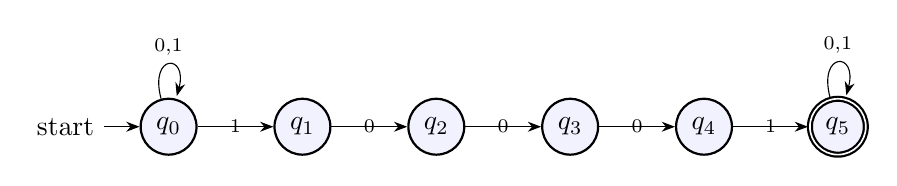
\begin{tikzpicture}[->, >=Stealth, node distance=1.7cm, every state/.style={thick, fill=blue!5, minimum size=0.7cm}]
    \node[state, initial]   (q0) {$q_0$};
    \node[state]            (q1) [right of=q0] {$q_1$};
    \node[state]            (q2) [right of=q1] {$q_2$};
    \node[state]            (q3) [right of=q2] {$q_3$};
    \node[state]            (q4) [right of=q3] {$q_4$};
    \node[state, accepting] (q5) [right of=q4] {$q_5$};

    \path (q0) edge [loop above] node {\scriptsize 0,1} ()
          (q0) edge              node {\scriptsize 1}   (q1)
          (q1) edge              node {\scriptsize 0}   (q2)
          (q2) edge              node {\scriptsize 0}   (q3)
          (q3) edge              node {\scriptsize 0}   (q4)
          (q4) edge              node {\scriptsize 1}   (q5)
          (q5) edge [loop above] node {\scriptsize 0,1} ();
\end{tikzpicture}
\end{center}

\textit{The nondeterminism: at $q_0$, reading 1, the machine can BOTH stay in $q_0$ (keep scanning) and go to $q_1$ (start verifying $10001$). It ``guesses'' where the substring starts.}

\textbf{Key theorem from Semester 1:} NFAs and DFAs recognize the same class of languages (regular languages). The NTM $\leftrightarrow$ DTM equivalence in this lecture is the \textit{same idea}, but for Turing machines.
\end{definitionbox}

%───────────────────────────────────────────────────────────────────────────────
\subsection{Definition: Nondeterministic Turing Machine (NTM) (slide 22) \kemark}

\begin{notebox}{Analogy: A GPS That Shows ALL Routes Simultaneously}
Imagine a GPS app that, at every intersection, doesn't pick one route --- it splits the screen and shows ALL possible routes continuing simultaneously. Each route proceeds independently. If \textit{any} route reaches the destination, the GPS says ``route found!''

\textbf{In our formal world:}
\begin{itemize}[nosep]
\item ``GPS'' = the NTM
\item ``Intersection with options'' = configuration where $\delta(q, a)$ has multiple elements
\item ``Each route'' = a branch in the computation tree
\item ``Destination'' = accepting state $t$
\item ``Route found'' = NTM accepts (at least one branch reaches $t$)
\end{itemize}
\end{notebox}

\begin{definitionbox}{Nondeterministic Turing Machine (NTM)}

\textbf{Plain English:} An NTM is like a DTM, but at each step, instead of having exactly one next move, it can have \textbf{multiple} possible next moves. The machine ``branches'' into all possibilities simultaneously.

\textbf{Formal:} An NTM has the form $(Q, \Sigma, \Gamma, s, t, r, \delta)$ where $Q, \Sigma, \Gamma, s, t, r$ are as for DTMs, and:

\fitmath{\delta\colon (Q \setminus \{t, r\}) \times \Gamma \to 2^{Q \times \Gamma \times \{-1, +1\}}}

\textbf{Breaking Down the Notation:}
\begin{itemize}[nosep]
\item $(Q \setminus \{t, r\}) \times \Gamma$ = the domain: current (non-halting) state and symbol under head
\item $2^{Q \times \Gamma \times \{-1, +1\}}$ = the codomain: the \textbf{power set} (= set of all subsets) of $Q \times \Gamma \times \{-1, +1\}$. This means $\delta(q, a)$ returns a \textbf{set} of (state, symbol, direction) triples.
\item If $\delta(q, a) = \{(q_1, b_1, d_1), (q_2, b_2, d_2)\}$, then from configuration $[q, \tau, \ell]$ there are TWO successor configurations.
\item A DTM is the special case where $|\delta(q, a)| = 1$ always.
\end{itemize}

\textbf{Comparison table --- DTM vs NTM:}
\begin{center}
\renewcommand{\arraystretch}{1.3}
\begin{tabular}{lp{5.5cm}p{5.5cm}}
\toprule
& \textbf{DTM} & \textbf{NTM} \\
\midrule
$\delta$ codomain & $Q \times \Gamma \times \{-1,+1\}$ (one triple) & $2^{Q \times \Gamma \times \{-1,+1\}}$ (a SET of triples) \\
\# of successor configs & Exactly 1 & 0 or more \\
Computation shape & Single path (like a line) & Tree (branches at each step) \\
Acceptance & Reaches $t$ & $\exists$ branch that reaches $t$ \\
Configurations & Same definition & Same definition \\
Initial config & Same & Same \\
\bottomrule
\end{tabular}
\end{center}

\textbf{Concrete example with $\{w\#w\}$:} A single-tape DTM for $\{w\#w\}$ deterministically picks the rightmost unmatched symbol and matches it. An NTM could \textit{nondeterministically} guess which position to check next, or guess that the entire string matches and then verify --- but this doesn't change what languages are computable.

\kt{The ONLY difference between a DTM and an NTM is the transition function's codomain: one triple (DTM) vs.\ a SET of triples (NTM). Everything else --- states, tapes, alphabet, configurations --- is identical.}

\textbf{Connection to Exercises:} Exercise 3 tests your understanding of NTM \textit{acceptance}. Exercise 4 asks you to \textit{construct} NTMs. Both require you to understand this definition deeply.
\end{definitionbox}

%───────────────────────────────────────────────────────────────────────────────
\subsection{The Computation Tree (slide 23) \kemark}

\begin{notebox}{Analogy: A ``Choose Your Own Adventure'' Book}
You start at page 1. Some pages give you choices: ``To fight the dragon, turn to page 42. To flee, turn to page 87.'' Each choice creates a branch. If you draw ALL possible reading paths from page 1, you get a \textbf{tree}. Some paths end with ``The End --- You Win!'' (accept). Some end with ``The End --- You Lose'' (reject). Some paths might go on forever (looping story).

\textbf{In our formal world:}
\begin{itemize}[nosep]
\item ``Page 1'' = the initial configuration $\alpha_w$
\item ``Choice at a page'' = $\delta(q, a)$ having multiple elements
\item ``Each reading path'' = one branch from root to leaf (or to infinity)
\item ``You Win!'' = accepting configuration (state $t$)
\item ``You Lose'' = rejecting configuration (state $r$)
\item ``Story goes on forever'' = infinite branch (looping computation)
\item ``Hero wins'' = the NTM accepts = there EXISTS at least one winning path
\end{itemize}
\end{notebox}

\begin{definitionbox}{Computation Tree of an NTM}

\textbf{Plain English:} The computation tree of NTM $M$ on input $w$ shows ALL possible computation paths, branching at every nondeterministic choice.

\textbf{Formal structure:}
\begin{itemize}[nosep]
\item \textbf{Root} = the initial configuration $\alpha_w$ (starting point)
\item \textbf{Children of node $\gamma$} = all successor configurations of $\gamma$ (one for each element in $\delta(q, a)$ where $\gamma = [q, \tau, \ell]$ and $a = \tau(\ell)$)
\item \textbf{Leaves} = halting configurations (accept $t$ or reject $r$)
\item \textbf{Infinite branches} = computation paths that never halt
\end{itemize}

\textbf{Visual example:} If $\delta(q, b) = \{(q_1, c, 0), (q_2, d, +1), (q_3, e, -1)\}$, then from $[q, \ldots]$ we get three children:

\begin{center}
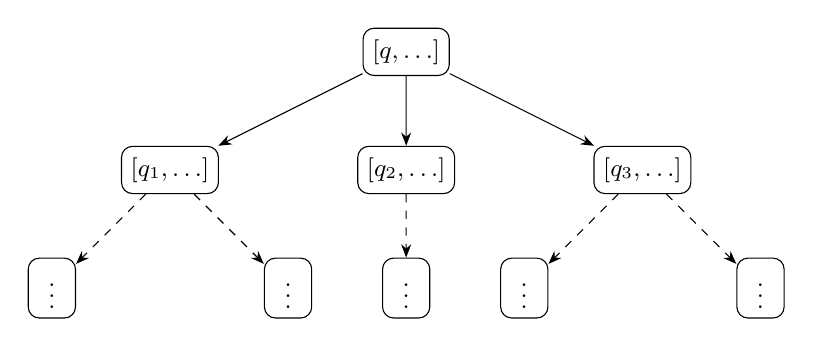
\begin{tikzpicture}[
    level distance=1.5cm,
    sibling distance=3cm,
    edge from parent/.style={draw, ->, >=Stealth},
    every node/.style={draw, rounded corners, minimum size=0.6cm, font=\small}
]
    \node {$[q, \ldots]$}
        child { node {$[q_1, \ldots]$}
            child { node {$\vdots$} edge from parent[dashed] }
            child { node {$\vdots$} edge from parent[dashed] }
        }
        child { node {$[q_2, \ldots]$}
            child { node {$\vdots$} edge from parent[dashed] }
        }
        child { node {$[q_3, \ldots]$}
            child { node {$\vdots$} edge from parent[dashed] }
            child { node {$\vdots$} edge from parent[dashed] }
        };
\end{tikzpicture}
\end{center}

\textbf{Breaking Down the Properties:}
\begin{itemize}[nosep]
\item The tree may be \textbf{infinite} (if any branch loops forever)
\item The \textbf{branching factor} at each node $\leq |\delta(q, a)|$ (bounded by the number of options)
\item Different branches are \textbf{independent} --- they don't interact or share information
\item Each root-to-leaf (or root-to-infinity) path is called a ``computation'' or ``run'' of the NTM
\end{itemize}

\kt{The computation tree is the key mental model for NTMs. Every ``run'' is one root-to-leaf path. The NTM ``explores'' the entire tree simultaneously. It accepts if ANY path reaches an accepting leaf.}
\end{definitionbox}

%───────────────────────────────────────────────────────────────────────────────
\subsection{NTM Acceptance (slide 24) \kemark}

\begin{notebox}{Analogy: University Applications}
You apply to 10 universities. You get accepted to 3 and rejected by 7. Are you ``accepted''? \textbf{Yes!} You only need ONE acceptance letter. You don't need all 10 to accept you. It doesn't matter that 7 rejected you.

\textbf{In our formal world:}
\begin{itemize}[nosep]
\item ``10 universities'' = 10 branches in the computation tree
\item ``3 accept you'' = 3 branches reach state $t$
\item ``7 reject you'' = 7 branches reach state $r$ (or loop forever)
\item ``Are you accepted?'' = does the NTM accept? YES --- at least one branch accepted.
\end{itemize}
\end{notebox}

\begin{definitionbox}{NTM Acceptance --- The ``Exists'' Rule}

\textbf{Plain English:} An NTM accepts input $w$ if there EXISTS at least one computation path that reaches the accepting state $t$. It doesn't matter if other paths reject or loop.

\textbf{Formal:}

An NTM $M$ \textbf{accepts} input $w$ if the computation tree of $M$ on $w$ contains at least one accepting configuration.

\fitmath{L(M) = \{w \in \Sigma^* \mid \exists \text{ a computation of } M \text{ on } w \text{ that halts in state } t\}}

\textbf{Breaking Down the Definition:}
\begin{itemize}[nosep]
\item $M$ \textbf{accepts} $w$ if $\exists$ at least one branch reaching $t$
\item $M$ \textbf{does NOT accept} $w$ if NO branch reaches $t$ (all branches reject or loop)
\item If some branches accept and some reject: the NTM \textbf{accepts} (``exists'' wins)
\item If some branches loop and none accepts: the NTM \textbf{does not accept} (and might loop forever trying to explore all branches in a simulation)
\end{itemize}

\textbf{Concrete example:} Consider an NTM for ``does input $w$ contain $110$?'' On input $w = 0110$:
\begin{itemize}[nosep]
\item Branch 1: guesses position 1, checks ``011'' --- not 110. \textbf{Rejects.}
\item Branch 2: guesses position 2, checks ``110'' --- yes! \textbf{Accepts!}
\item Branch 3: guesses position 3, checks ``10$\sqcup$'' --- not 110. \textbf{Rejects.}
\item Branch 4: keeps scanning, never guesses. \textbf{Rejects} (hits blank).
\end{itemize}
At least one branch (Branch 2) accepts $\Rightarrow$ the NTM accepts $0110$.

\kt{NTM acceptance = ``there EXISTS at least one computation that halts in state $t$.'' Not ``all,'' not ``most,'' not ``exactly one'' --- just ``at least one.'' This is the single most tested concept from this lecture.}

\textbf{Connection to Exercises:} Exercise 3 directly tests this. You must identify which of 5 statements correctly defines NTM acceptance.
\end{definitionbox}

%───────────────────────────────────────────────────────────────────────────────
\subsection{Exercise 3: Test Your Understanding of NTM Acceptance \kemark}

\begin{conceptbox}{{WARNING: The Five Definitions (Exercise 3) --- Which Is Correct?}}

Exercise 3 presents five statements. Only \textbf{one} is correct. Here's each one with a verdict and explanation:

\renewcommand{\arraystretch}{1.5}
\begin{center}
\begin{tabular}{cp{7cm}cc}
\toprule
\textbf{\#} & \textbf{Statement} & \textbf{Verdict} & \textbf{Why} \\
\midrule
1 & $M$ accepts $w$ if $\exists$ \textbf{more than one} computation halting in $t$ & \textcolor{red}{\textbf{WRONG}} & One is enough \\
2 & $M$ accepts $w$ if \textbf{no} computation halts in $r$ & \textcolor{red}{\textbf{WRONG}} & All could loop \\
3 & $M$ accepts $w$ if $\exists$ \textbf{a} computation halting in $t$ & \textcolor{green!60!black}{\textbf{RIGHT}} & Correct definition \\
4 & $M$ accepts $w$ if $\exists$ \textbf{exactly one} accepting computation & \textcolor{red}{\textbf{WRONG}} & Multiple is fine \\
5 & $M$ accepts $w$ if \textbf{every} computation halts in $t$ & \textcolor{red}{\textbf{WRONG}} & Too strong \\
\bottomrule
\end{tabular}
\end{center}

\textbf{Detailed explanations of why each wrong answer fails:}

\textbf{\#1 --- ``more than one'':} Suppose the NTM has exactly one computation that accepts. By the real definition, the NTM accepts. Statement \#1 says it doesn't (because we need ``more than one''). So \#1 is wrong --- one accepting computation is sufficient.

\textbf{\#2 --- ``no computation halts in $r$'':} Suppose all computations loop forever (none halts in $r$, but none halts in $t$ either). Statement \#2 says the NTM accepts (because no computation halts in $r$). But the real definition says the NTM does NOT accept (because no computation reaches $t$). No accepting configuration is reached, so the machine rejects (or more precisely, doesn't accept).

\textbf{\#3 --- ``there exists a computation halting in $t$'':} This is exactly the definition. The NTM accepts $w$ $\Leftrightarrow$ $\exists$ at least one path in the computation tree that reaches $t$. \textbf{Correct.}

\textbf{\#4 --- ``exactly one'':} Suppose two branches both accept. By the real definition, the NTM accepts. Statement \#4 says it doesn't (because there isn't \textit{exactly} one). There can be any number of accepting branches --- what matters is $\geq 1$.

\textbf{\#5 --- ``every computation'':} This requires ALL branches to accept. But the real definition only requires at least one. If 99 branches reject and 1 accepts, the NTM accepts. Statement \#5 would say it doesn't.

\kt{The correct answer is \textbf{\#3}: ``$M$ accepts $w$ if there exists a computation of $M$ on $w$ such that $M$ halts in state $t$.'' The key word is ``\textbf{exists}'' --- existential, not universal.}
\end{conceptbox}

%───────────────────────────────────────────────────────────────────────────────
\subsection{Halting NTM (slide 24) \kemark}

\begin{notebox}{Analogy: A ``Choose Your Own Adventure'' Where Every Story Ends}
Some adventure books have infinite loops (``go back to page 1 forever''). A ``halting'' adventure book is one where \textit{every} possible storyline eventually reaches ``The End'' --- no infinite loops, no matter what choices you make.

\textbf{In our formal world:}
\begin{itemize}[nosep]
\item ``Every storyline eventually ends'' = every branch of the computation tree reaches $t$ or $r$
\item ``Halting adventure book'' = halting NTM
\item ``No infinite loops'' = computation tree is finite
\end{itemize}
\end{notebox}

\begin{definitionbox}{Halting NTM}

\textbf{Plain English:} A halting NTM is an NTM where, for every input $w$, the computation tree is \textbf{finite}. Every branch eventually reaches $t$ or $r$. No branch loops forever.

\textbf{Formal:} An NTM $M$ is a \textbf{halting NTM} if for every input $w$, the computation tree of $M$ on $w$ is finite (i.e., every branch has finite length).

\textbf{Breaking Down What This Means:}
\begin{itemize}[nosep]
\item ``Computation tree is finite'' = ALL branches terminate (reach $t$ or $r$), not just some
\item In a halting NTM: $M$ accepts $w$ $\Leftrightarrow$ at least one leaf is $t$; $M$ rejects $w$ $\Leftrightarrow$ ALL leaves are $r$
\end{itemize}

\textbf{Concrete example:} Our NTM for ``contains 110'' (Section 5.8) is a halting NTM --- every branch either reaches $t$ (found 110) or reaches $r$ (wrong guess or end of input). No branch loops.

\kt{``Halting NTM'' means the ENTIRE computation tree is finite (ALL branches terminate), not just that some branch terminates. Compare: ``halting DTM'' means the single computation path terminates.}

\textbf{Connection to Exercises:} The NTMs you build in Exercise 4 should be halting NTMs (every branch terminates). This is analogous to building halting DTMs for computable languages.
\end{definitionbox}


%───────────────────────────────────────────────────────────────────────────────
\subsection{Constructing NTMs --- The ``Guess and Verify'' Pattern (Exercise 4) \kemark}

\begin{notebox}{Analogy: A Multiple-Choice Exam Where You Circle ALL Answers}
Imagine a multiple-choice exam where, instead of picking one answer, you circle ALL options simultaneously. A grader checks every circled answer. If \textit{any} one of them is correct, you get the mark.

\textbf{In our formal world:}
\begin{itemize}[nosep]
\item ``Circling all options'' = nondeterministic branching (trying all possibilities)
\item ``Grader checks'' = each branch runs its deterministic verification
\item ``Any one correct'' = at least one branch accepts
\item ``Get the mark'' = the NTM accepts the input
\end{itemize}

This is the \textbf{``guess and verify''} pattern: nondeterministically GUESS a ``certificate'' (a potential answer), then deterministically VERIFY it.
\end{notebox}

\begin{examplebox}{{Exercise 4.1: NTM for $L = \{w \in \{0,1\}^* \mid w$ contains infix $110\}$}}

\textbf{Strategy:}
\begin{enumerate}[nosep]
\item \textbf{Guess:} Nondeterministically guess WHERE the infix $110$ starts (by choosing to leave the ``scanning'' state at some position)
\item \textbf{Verify:} Deterministically check that the next three symbols are $1, 1, 0$
\end{enumerate}

\textbf{Formal definition:} $M = (Q, \Sigma, \Gamma, s, t, r, \delta)$ with:
\begin{itemize}[nosep]
\item $Q = \{s, t, r, q_1, q_{11}\}$
\item $\Sigma = \{0, 1\}$
\item $\Gamma = \{0, 1, \sqcup\}$
\item $\delta$ given by the table below:
\end{itemize}

\begin{center}
\renewcommand{\arraystretch}{1.3}
\begin{tabular}{llp{7cm}}
\toprule
State & Read & $\delta(\text{state, read})$ \\
\midrule
$s$ & 0 & $\{(s, 0, +1)\}$ \quad keep scanning, didn't see 1 \\
$s$ & 1 & $\{(s, 1, +1),\; (q_1, 1, +1)\}$ \quad \textbf{BRANCH}: keep scanning OR start verifying \\
$s$ & $\sqcup$ & $\{(r, \sqcup, +1)\}$ \quad end of input, never started verifying: reject \\
\midrule
$q_1$ & 0 & $\{(r, 0, -1)\}$ \quad needed 1, got 0: wrong guess, reject branch \\
$q_1$ & 1 & $\{(q_{11}, 1, +1)\}$ \quad got second 1, continue \\
$q_1$ & $\sqcup$ & $\{(r, \sqcup, +1)\}$ \quad end of input: reject branch \\
\midrule
$q_{11}$ & 0 & $\{(t, 0, +1)\}$ \quad \textbf{FOUND 110! ACCEPT!} \\
$q_{11}$ & 1 & $\{(r, 1, +1)\}$ \quad needed 0, got 1: wrong guess, reject branch \\
$q_{11}$ & $\sqcup$ & $\{(r, \sqcup, +1)\}$ \quad end of input: reject branch \\
\bottomrule
\end{tabular}
\end{center}

\textbf{State diagram:}
\begin{center}
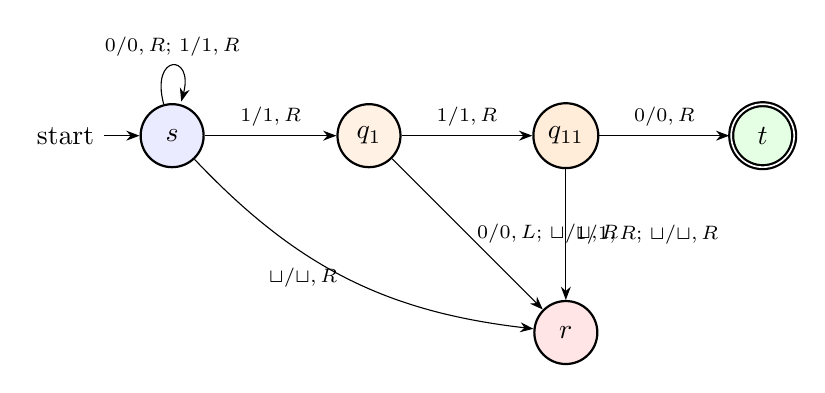
\begin{tikzpicture}[->, >=Stealth, node distance=2.5cm, every state/.style={thick, minimum size=0.8cm}]
    \node[state, initial, fill=blue!8]      (s)   {$s$};
    \node[state, fill=orange!10]            (q1)  [right of=s] {$q_1$};
    \node[state, fill=orange!15]            (q11) [right of=q1] {$q_{11}$};
    \node[state, accepting, fill=green!10]  (t)   [right of=q11] {$t$};
    \node[state, fill=red!10]               (r)   [below of=q11] {$r$};

    \path (s)   edge [loop above] node {\scriptsize $0/0,R$; $1/1,R$} ()
          (s)   edge              node [above] {\scriptsize $1/1,R$} (q1)
          (q1)  edge              node [above] {\scriptsize $1/1,R$} (q11)
          (q11) edge              node [above] {\scriptsize $0/0,R$} (t)
          (s)   edge [bend right=20] node [left] {\scriptsize $\sqcup/\sqcup,R$} (r)
          (q1)  edge              node [right] {\scriptsize $0/0,L$; $\sqcup/\sqcup,R$} (r)
          (q11) edge              node [right] {\scriptsize $1/1,R$; $\sqcup/\sqcup,R$} (r);
\end{tikzpicture}
\end{center}

\textit{The nondeterminism: the double arrow from $s$ on reading 1 --- one branch stays in $s$ (``not yet''), the other goes to $q_1$ (``I think 110 starts here'').}

\textbf{Concrete trace on input $w = 0110$:}

\begin{lstlisting}
Level 0: [s, 0110, pos=1]                       % initial configuration
  Read 0 -> only option: stay in s
Level 1: [s, 0110, pos=2]
  Read 1 -> BRANCH! Two successors:
    Level 2a: [s, 0110, pos=3]                   % kept scanning
      Read 1 -> BRANCH again:
        Level 3a: [s, 0110, pos=4]               % kept scanning
          Read 0 -> stay in s
            Level 4a: [s, 0110_, pos=5]
              Read _ -> REJECT (branch dies)
        Level 3b: [q1, 0110, pos=4]              % started verifying at pos 3
          Read 0 -> needed 1, got 0 -> REJECT (branch dies)
    Level 2b: [q1, 0110, pos=3]                  % started verifying at pos 2
      Read 1 -> go to q11
        Level 3c: [q11, 0110, pos=4]
          Read 0 -> ACCEPT! (state t reached!)
\end{lstlisting}

Branch 3c reaches $t$ $\Rightarrow$ the NTM accepts $0110$. The other branches that rejected don't matter.

\textbf{Trace on input $w = 0010$ (does NOT contain 110):}

Every branch where $s$ transitions to $q_1$ eventually rejects (none of them find $1, 1, 0$ in sequence). The branch that stays in $s$ forever also rejects (hits blank). ALL branches reject $\Rightarrow$ the NTM rejects $0010$.

\kt{The ``guess and verify'' pattern: use nondeterminism to guess WHERE something interesting happens (the NTM ``clones itself'' at every potential start position), then verify deterministically. The NTM accepts if ANY guess turns out correct.}
\end{examplebox}

%───────────────────────────────────────────────────────────────────────────────
\subsection{Exercise 4.2: NTM for Composite Numbers \kemark}

\begin{notebox}{Analogy: Guessing the Factors of a Number}
You want to check if a number $n$ is composite (not prime). A deterministic approach: try every divisor from 2 to $\sqrt{n}$. A nondeterministic approach: \textbf{guess} two numbers $n_0, n_1 > 1$, multiply them, and check if the result equals $n$. If any guess gives $n_0 \cdot n_1 = n$, then $n$ is composite.

\textbf{In our formal world:}
\begin{itemize}[nosep]
\item ``Guess two numbers'' = nondeterministically choose $n_0, n_1$
\item ``Multiply and check'' = deterministic verification
\item ``Result equals $n$'' = accepting branch
\end{itemize}
\end{notebox}

\begin{examplebox}{{NTM for $L = \{a^n \mid n$ is composite$\}$}}

\textbf{Input:} A string $a^n$ (n copies of letter $a$). Question: is $n$ composite?

\textbf{Strategy:}
\begin{enumerate}[nosep]
\item \textbf{Guess:} Nondeterministically guess two numbers $n_0, n_1$ with $1 < n_0 \leq n$ and $1 < n_1 \leq n$
\item \textbf{Verify:} Compute $n_0 \cdot n_1$ (e.g., using a multi-tape NTM --- we know multi-tape is equivalent)
\item \textbf{Compare:} If $n_0 \cdot n_1 = n$, accept. Otherwise, reject this branch.
\end{enumerate}

\textbf{Why this works:}
\begin{itemize}[nosep]
\item If $n$ is composite: $\exists\; n_0, n_1 > 1$ with $n_0 \cdot n_1 = n$. The NTM can guess these, and that branch accepts.
\item If $n$ is prime (or $\leq 1$): no such $n_0, n_1$ exist. ALL guesses fail. ALL branches reject.
\end{itemize}

\textbf{Concrete example:} Input $a^6$ (i.e., $n = 6$).
\begin{itemize}[nosep]
\item Branch guessing $n_0 = 2, n_1 = 3$: computes $2 \times 3 = 6 = n$. \textbf{ACCEPT!}
\item Branch guessing $n_0 = 2, n_1 = 2$: computes $2 \times 2 = 4 \neq 6$. Reject.
\item Branch guessing $n_0 = 3, n_1 = 3$: computes $3 \times 3 = 9 \neq 6$. Reject.
\item \ldots many other branches, all rejecting. But at least one accepts $\Rightarrow$ NTM accepts $a^6$.
\end{itemize}

Input $a^5$ (i.e., $n = 5$, prime): every guess fails. No $n_0, n_1 > 1$ multiply to 5. ALL branches reject $\Rightarrow$ NTM rejects $a^5$.

\kt{Nondeterminism is powerful for ``search'' problems: guess the certificate (the factors), verify deterministically (multiply and compare). The NTM ``finds'' the factors without searching --- it tries ALL possibilities at once.}
\end{examplebox}


%═══════════════════════════════════════════════════════════════════════════════
\newpage
\section{The NTM Simulation Theorem (slide 25) \kemark}
%═══════════════════════════════════════════════════════════════════════════════

\begin{notebox}{Analogy: A Systematic Chess Player vs.\ a ``See the Future'' Player}
Imagine a chess player who can ``see the future'' --- simultaneously exploring ALL possible move sequences. You, as a human, can only try one sequence at a time. But if you're systematic (check all 1-move sequences, then all 2-move sequences, then all 3-move sequences\ldots), you'll eventually find any winning sequence the ``future-seer'' would find. You're much slower, but you explore the same space.

\textbf{In our formal world:}
\begin{itemize}[nosep]
\item ``See the future player'' = NTM (explores all branches simultaneously)
\item ``Systematic player'' = DTM doing BFS of the computation tree
\item ``1-move, 2-move, 3-move sequences'' = computation tree levels 1, 2, 3
\item ``Find any winning sequence'' = find any accepting configuration
\end{itemize}
\end{notebox}

\begin{definitionbox}{{Theorem: Every NTM Can Be Simulated by a DTM}}

\textbf{Plain English:} For every NTM $M$, there exists a standard DTM $M'$ that outcome-simulates $M$. Nondeterminism does NOT add computational power.

\textbf{Formal:}
\begin{center}
\fbox{\parbox{0.85\linewidth}{\centering For every NTM $M$ there is a (standard, deterministic) DTM $M'$ that outcome-simulates $M$.}}
\end{center}

\textbf{The simulation algorithm --- BFS of the computation tree:}

This algorithm systematically explores the computation tree level by level. It maintains a set $\Gamma_i$ of all configurations reachable in exactly $i$ steps, checks each level for acceptance, and computes the next level by finding all successor configurations.

\begin{lstlisting}
def simulate_NTM(M, w):                       % Input: NTM M, input word w
    alpha_w = initial_config(M, w)             % Build initial config of M on w
    Gamma_0 = {alpha_w}                        % Level 0: just the initial config
    i = 0                                      % Start at level 0
    while True:                                % Loop forever (until halt)
        if any config in Gamma_i is accepting: % Check: does level i have state t?
            return ACCEPT                      % Found accepting config -> accept!
        if Gamma_i is empty:                   % Check: no configs left at all?
            return REJECT                      % All branches halted without accepting
        Gamma_{i+1} = {}                       % Prepare next level
        for each gamma in Gamma_i:             % For every config at current level
            for each gamma' with               % Find ALL successor configs
                gamma |-_M gamma':             %   (one for each element of delta)
                add gamma' to Gamma_{i+1}      % Add successor to next level
        i = i + 1                              % Move to next level
\end{lstlisting}

\textbf{Tracing the algorithm on our NTM for ``contains 110'' on input $0110$:}

\begin{lstlisting}
Gamma_0 = {[s, 0110, 1]}                     % Initial config

Level 0: No accepting config. Not empty. Compute successors.
  [s, 0110, 1]: read 0 -> {(s,0,+1)} -> successor: [s, 0110, 2]
Gamma_1 = {[s, 0110, 2]}

Level 1: No accepting. Not empty. Compute successors.
  [s, 0110, 2]: read 1 -> {(s,1,+1), (q1,1,+1)} -> 2 successors!
Gamma_2 = {[s, 0110, 3], [q1, 0110, 3]}

Level 2: No accepting. Not empty.
  [s, 0110, 3]: read 1 -> {(s,1,+1), (q1,1,+1)} -> 2 successors
  [q1, 0110, 3]: read 1 -> {(q11,1,+1)} -> 1 successor
Gamma_3 = {[s, 0110, 4], [q1, 0110, 4], [q11, 0110, 4]}

Level 3: Check each config:
  [s, 0110, 4]: state s, not accepting
  [q1, 0110, 4]: state q1, not accepting
  [q11, 0110, 4]: read 0 -> {(t,0,+1)} -> successor has state t!
  But wait -- we check Gamma_3 for accepting, and q11 isn't t.
  Compute Gamma_4:
  [s, 0110, 4]: read 0 -> {(s,0,+1)} -> [s, 0110_, 5]
  [q1, 0110, 4]: read 0 -> {(r,0,-1)} -> [r, ...] (reject leaf)
  [q11, 0110, 4]: read 0 -> {(t,0,+1)} -> [t, 0110, 5]
Gamma_4 = {[s, 0110_, 5], [t, 0110, 5]}  (reject leaf excluded)

Level 4: [t, 0110, 5] is accepting! -> ACCEPT!
\end{lstlisting}

\textbf{Why BFS and not DFS?}

\textit{If we used depth-first search instead:} Suppose branch A goes infinitely deep (loops forever) and branch B accepts at depth 3. DFS might explore branch A forever and \textbf{never discover} branch B. The simulation would loop even though the NTM accepts!

BFS guarantees fairness: we check ALL branches at depth $d$ before going to depth $d+1$. If any branch accepts at depth $d$, we find it at level $d$. We never get ``stuck'' in an infinite branch.

\textbf{Corollary:}
\begin{enumerate}[nosep]
\item A language is computably-enumerable $\Leftrightarrow$ it is the language of some NTM
\item A language is computable $\Leftrightarrow$ it is the language of some halting NTM
\end{enumerate}

\kt{The DTM simulates the NTM by doing BFS of the computation tree: explore level 0, then level 1, then level 2, etc. Check each level for an accepting configuration. BFS is required because DFS can get stuck in infinite branches.}
\end{definitionbox}


%═══════════════════════════════════════════════════════════════════════════════
\newpage
\section{Robustness Deep-Dive: The Doubly-Infinite Tape (Exercise 2) \kemark}
%═══════════════════════════════════════════════════════════════════════════════

\begin{notebox}{Analogy: A Two-Way Street vs.\ a One-Way Street}
A standard TM's tape is like a one-way street with a dead end: you can drive forward (right) forever, but there's a wall at the left end (position 1). A doubly-infinite tape is like a two-way street that extends forever in both directions --- no wall, no dead end.

\textbf{In our formal world:}
\begin{itemize}[nosep]
\item ``Dead end on the left'' = singly-infinite tape has a leftmost cell (position 1)
\item ``Two-way street'' = doubly-infinite tape has cells at positions $\ldots, -2, -1, 0, 1, 2, \ldots$
\item ``Same destinations'' = same computable languages
\end{itemize}

Exercise 2 asks three things: (1) formally define the doubly-infinite tape DTM, (2) show singly-infinite can simulate doubly-infinite, (3) show doubly-infinite can simulate singly-infinite.
\end{notebox}

%───────────────────────────────────────────────────────────────────────────────
\subsection{Part 1: Formal Definition of a Doubly-Infinite Tape DTM}

\begin{definitionbox}{{DTM with Doubly-Infinite Tape}}

\textbf{Plain English:} Same $(Q, \Sigma, \Gamma, s, t, r, \delta)$ tuple as a standard DTM. The only difference is in the \textit{semantics}: how configurations work (cells indexed by ALL integers, not just positive ones) and how successor configurations work (no special case for ``head at leftmost cell'').

\textbf{Formal:} A configuration is a triple $[q, \tau, \ell]$ where:
\begin{itemize}[nosep]
\item $q \in Q$ = current state
\item $\tau\colon \mathbb{Z} \to \Gamma$ = tape content (indexed by \textbf{all integers}, positive AND negative)
\item $\ell \in \mathbb{Z}$ = head position (can be any integer)
\end{itemize}

\textbf{Breaking Down the Notation:}
\begin{itemize}[nosep]
\item $\mathbb{Z}$ (not $\mathbb{N}$!) = the tape has cells at positions $\ldots, -2, -1, 0, 1, 2, \ldots$
\item $\tau\colon \mathbb{Z} \to \Gamma$ = every integer position has a symbol. Initially, positions outside the input are $\sqcup$.
\item $\ell \in \mathbb{Z}$ = the head can be at ANY position, including negative ones
\end{itemize}

\textbf{Initial configuration on $w = w_1 \ldots w_k$:} $[s, \tau, 1]$ where:
\fitmath{\tau(n) = \begin{cases} w_n & \text{if } n \in \{1, \ldots, k\} \\ \sqcup & \text{otherwise (including negative positions)} \end{cases}}

\textbf{Successor configuration:} Given $[q, \tau, \ell]$ with $\delta(q, \tau(\ell)) = (p, a, d)$:

The successor is $[p, \tau', \ell + d]$ where $\tau'(n) = a$ if $n = \ell$, and $\tau'(n) = \tau(n)$ otherwise.

\textbf{Key difference from singly-infinite:} No special case for ``head at position 1 trying to go left.'' The head can \textbf{always} go left --- there's no boundary to get stuck at.

\textbf{Concrete example with $\{w\#w\}$:} On input $01\#01$, the initial config is $[s, \tau, 1]$ with $\tau(1)=0, \tau(2)=1, \tau(3)=\#, \tau(4)=0, \tau(5)=1$, and $\tau(n)=\sqcup$ for all other $n$ (including $n=0, -1, -2, \ldots$). The machine could move left to position 0 or $-1$ --- it would just find blanks there.

\kt{A doubly-infinite tape DTM has the exact same tuple as a standard DTM. The only change is the configuration definition: cells indexed by $\mathbb{Z}$ instead of $\mathbb{N}$, and no left-boundary special case.}
\end{definitionbox}

%───────────────────────────────────────────────────────────────────────────────
\subsection{Part 2: Singly-Infinite Simulates Doubly-Infinite}

\begin{notebox}{Analogy: Fitting a Two-Way Street onto a One-Way Street}
You have a two-way street (traffic goes left and right) but need to fit it onto a one-way street (traffic only goes right). Solution: place cones at the boundary, and whenever a car needs to go ``left'' past the boundary, shift all the cars one space to the right to make room.

\textbf{In our formal world:}
\begin{itemize}[nosep]
\item ``Cones at boundary'' = markers $\ell$ (left end) and $r$ (right end) on the tape
\item ``Shift cars right'' = shift all tape content one cell right when the head needs to go left past the boundary
\end{itemize}
\end{notebox}

\begin{examplebox}{{Simulation: Doubly-Infinite $\to$ Singly-Infinite}}

\textbf{The challenge:} A doubly-infinite tape has cells at $\ldots, -2, -1, 0, 1, 2, \ldots$ but a singly-infinite tape only has $1, 2, 3, \ldots$ How do we handle the ``negative'' cells?

\textbf{The construction:} $M'$ uses two special markers (not in $M$'s tape alphabet):
\begin{itemize}[nosep]
\item $\ell$ = left boundary marker (marks the leftmost ``used'' cell)
\item $r$ = right boundary marker (marks the rightmost ``used'' cell)
\end{itemize}

\textbf{The algorithm:}
\begin{enumerate}[nosep]
\item Replace input $w$ on tape by $\ell\, w\, r$ (put markers around it). Move head to position of first letter (cell 2).
\item Simulate $M$'s transitions normally.
\item If accepting/rejecting state of $M$ reached: accept/reject.
\item If head reaches cell with $\ell$ (needs to go further left): shift ALL tape content from $\ell$ to $r$ one cell to the right, creating a new blank cell after $\ell$. Place head on that new blank cell.
\item If head reaches cell with $r$ (needs more space on the right): replace $r$ by $\sqcup$, write $r$ one cell further right.
\end{enumerate}

\textbf{Concrete example:}

Suppose $M$ is running on input $01$ and moves left past the original position 1.
\begin{lstlisting}
Initially:   [ l | 0 | 1 | r | _ | _ | ... ]
                   ^                             Head at position 2, state q

M moves left to position 1 (the l marker):
             [ l | 0 | 1 | r | _ | _ | ... ]
               ^                                 Head hits l!

Shift everything right:
             [ l | _ | 0 | 1 | r | _ | ... ]
                   ^                             New blank cell created!
                                                 Head on the new blank cell.

Now M can continue operating on this blank cell as if it were
position 0 of the doubly-infinite tape.
\end{lstlisting}

\textbf{Why it's correct:} $M'$ always maintains a ``window'' of used cells between $\ell$ and $r$. Whenever $M$ would go to a cell outside the window, $M'$ expands the window by shifting. The shift is expensive ($O(n)$ per expansion) but finite.

\kt{Simulate left-expansion of a doubly-infinite tape on a singly-infinite tape by shifting content right when the head hits the left boundary. More steps, same answers.}
\end{examplebox}

%───────────────────────────────────────────────────────────────────────────────
\subsection{Part 3: Doubly-Infinite Simulates Singly-Infinite}

\begin{examplebox}{{Simulation: Singly-Infinite $\to$ Doubly-Infinite}}

\textbf{This direction is easier:} A doubly-infinite tape ``contains'' a singly-infinite tape (cells $1, 2, 3, \ldots$ exist on both). The only problem: on a singly-infinite tape, the head \textit{stays put} when at position 1 and trying to go left. On a doubly-infinite tape, it would go to position 0.

\textbf{The trick:} Place a special marker $\#$ at position 0 (just left of the input). Whenever the head hits $\#$, bounce back right.

\textbf{Formally:} Given singly-infinite DTM $M = (Q, \Sigma, \Gamma, s, t, r, \delta)$, construct doubly-infinite DTM $M' = (Q', \Sigma, \Gamma \cup \{\#\}, s', t, r, \delta')$:

\begin{itemize}[nosep]
\item $Q' = Q \cup \{s', q_\#\}$ (two new states for initialization)
\item \textbf{Initialization:}
  \begin{itemize}[nosep]
  \item $\delta'(s', a) = (q_\#, a, -1)$: move head left to position 0
  \item $\delta'(q_\#, \sqcup) = (s, \#, +1)$: place $\#$ marker at position 0, move right to the input, enter $M$'s start state
  \end{itemize}
\item \textbf{Normal operation:} $\delta'(q, a) = \delta(q, a)$ for all $q \in Q \setminus \{t,r\}$, $a \in \Gamma$
\item \textbf{Boundary handling:} $\delta'(q, \#) = (q, \#, +1)$ for all $q \in Q \setminus \{t,r\}$: if head reaches $\#$, bounce right (simulating the ``can't go left of position 1'' behavior)
\end{itemize}

\textbf{Concrete example:}
\begin{lstlisting}
Singly-infinite M on input 01:
  Tape: [ 0 | 1 | _ | _ | ... ]     Head at 1, trying to go left
         ^
  Can't go left! Head stays at position 1.

Doubly-infinite M' on input 01:
  After init: [ ... | # | 0 | 1 | _ | ... ]
                       ^                      Head at position 1, state s
  M' moves left to position 0:
              [ ... | # | 0 | 1 | _ | ... ]
                 ^                            Head reads #!
  delta'(q, #) = (q, #, +1): bounce back right:
              [ ... | # | 0 | 1 | _ | ... ]
                       ^                      Back at position 1!
\end{lstlisting}

Net effect: same as the singly-infinite tape's ``head stays put at left boundary.''

\kt{Together, Parts 2 and 3 prove: singly-infinite and doubly-infinite tapes compute the \textbf{same} languages. DTMs are robust with respect to tape boundaries.}
\end{examplebox}


%═══════════════════════════════════════════════════════════════════════════════
\newpage
\section{The Big Summary: All Models Are Equivalent}
%═══════════════════════════════════════════════════════════════════════════════

\begin{conceptbox}{The Robustness Landscape}

\textbf{Everything we proved in this lecture:}

\begin{center}
\renewcommand{\arraystretch}{1.4}
\begin{tabular}{lcp{6cm}}
\toprule
\textbf{Extension} & \textbf{More powerful?} & \textbf{How we proved it} \\
\midrule
``Stay'' direction (Ex 1) & No & Right-then-left with auxiliary state $q_L$ \\
$k$ tapes & No & Interleave on one tape, hat-marked heads \\
Nondeterminism & No & BFS of computation tree \\
Doubly-infinite tape (Ex 2) & No & Boundary markers + shifting / $\#$ marker \\
\midrule
\multicolumn{3}{l}{\textit{Not proved here but stated (Church-Kleene-Turing theorem):}} \\
$\lambda$-calculus & No & Formal proof of equivalence \\
$\mu$-recursive functions & No & Formal proof of equivalence \\
Python/Java/etc. & No & Church-Turing Thesis (claim) \\
\bottomrule
\end{tabular}
\end{center}

\textbf{What this means for our running example $\{w\#w\}$:} We can solve it with a single-tape DTM (L1), a 2-tape DTM (faster, Section 4), an NTM, a $\lambda$-calculus expression, a Python program, or even a Minecraft redstone circuit. All equivalent in \textit{what} they can compute, different in \textit{how fast} they compute it.

\kt{Turing machines are robust: adding tapes, nondeterminism, stay moves, or extending the tape doesn't change what's computable. This robustness is the strongest evidence for the Church-Turing Thesis.}
\end{conceptbox}


%═══════════════════════════════════════════════════════════════════════════════
\newpage
\section{Summary and Key Takeaways}
%═══════════════════════════════════════════════════════════════════════════════

\subsection{What We Learned (Big Picture)}

\begin{enumerate}
\item \textbf{The Church-Turing Thesis} \kbg{}: every reasonable formalization of computation is equivalent to TMs. It's a thesis (well-supported claim), not a theorem (mathematical proof).

\item \textbf{Turing-completeness} \kemark{}: a system is Turing-complete if it can simulate every TM. Java, Python, Excel, Minecraft --- all Turing-complete.

\item \textbf{Robustness} \kemark{}: no reasonable extension increases TM power. Proved for: stay moves (Exercise 1), multi-tape, nondeterminism, doubly-infinite tape (Exercise 2).

\item \textbf{Multi-tape DTMs} \kemark{}: $k$ independent tapes, one shared state. Simulated by interleaving tapes on one tape with an enlarged alphabet and hat-marked head positions.

\item \textbf{NTMs} \kemark{}: transition function returns a SET of options (branching). Accepts if ANY branch reaches $t$. Simulated by a DTM doing BFS of the computation tree.
\end{enumerate}

\subsection{Key Concepts Recap}

\begin{center}
\renewcommand{\arraystretch}{1.3}
\begin{tabular}{lp{9cm}}
\toprule
\textbf{Concept} & \textbf{One-Liner} \\
\midrule
Church-Turing Thesis & Everything computable can be computed by a TM (claim, not theorem) \\
Turing-complete & Can simulate every TM $=$ maximum computational power \\
Robust & No reasonable extension adds computational power \\
Outcome-simulation & $M'$ halts iff $M$ halts, and accepts iff $M$ accepts, on all inputs \\
$k$-tape DTM & $k$ tapes, 1 state; $\delta$ reads/writes $k$ symbols per step \\
NTM & Like DTM but $\delta$ returns a SET of triples; computation is a tree \\
NTM acceptance & $\exists$ at least one branch reaching $t$ (existential, not universal) \\
Halting NTM & ALL branches terminate (entire tree is finite) \\
Computation tree & Tree of all possible NTM paths on a given input \\
Guess and verify & NTM pattern: guess certificate, verify deterministically \\
\bottomrule
\end{tabular}
\end{center}

\subsection{Practical Guidelines for Exercises}

\begin{enumerate}[nosep]
\item \textbf{To prove robustness (Ex 1, 2):} Define a simulation from the ``fancy'' model to a standard DTM. Show it preserves halting and acceptance (= outcome-simulation).
\item \textbf{To build an NTM (Ex 4):} Use ``guess and verify'' --- nondeterministically guess a certificate, then deterministically verify it.
\item \textbf{To simulate an NTM:} Use BFS (NOT DFS!) of the computation tree.
\item \textbf{Multi-tape TMs in exercises:} Free to use (we proved they don't add power), treated as syntactic sugar.
\item \textbf{``Stay'' direction in exercises:} Free to use (we proved it's simulable).
\end{enumerate}

\subsection{Common Pitfalls and How to Avoid Them}

\begin{itemize}
\item \textbf{Pitfall:} ``NTMs are more powerful than DTMs.''

\textbf{Fix:} NTMs compute the \textbf{same} languages. They might be faster (relevant for NP in Lectures 6--7), but not more powerful in terms of computability.

\item \textbf{Pitfall:} ``NTM acceptance means ALL branches accept.''

\textbf{Fix:} Acceptance = EXISTS at least one accepting branch. One branch accepting is enough, even if 999 branches reject.

\item \textbf{Pitfall:} ``Nondeterminism = randomness.''

\textbf{Fix:} Nondeterminism explores ALL options simultaneously. Randomness picks ONE option with some probability. Completely different concepts.

\item \textbf{Pitfall:} ``The Church-Turing Thesis is proven.''

\textbf{Fix:} It's a \textit{thesis} (well-supported claim), not a theorem. It could theoretically be refuted.

\item \textbf{Pitfall:} ``Multi-tape TMs can compute languages that single-tape TMs can't.''

\textbf{Fix:} Same computational power. Multi-tape adds convenience and speed, not new capabilities.

\item \textbf{Pitfall:} ``Simulating an NTM with DFS works just as well as BFS.''

\textbf{Fix:} DFS can get stuck in an infinite branch and miss an accepting branch at a shallow depth. BFS is REQUIRED for correctness.
\end{itemize}

\subsection{Quick Reference: Simulation Techniques}

\begin{center}
\renewcommand{\arraystretch}{1.3}
\begin{tabular}{lp{9cm}}
\toprule
\textbf{Simulate\ldots} & \textbf{How} \\
\midrule
Stay direction & Right-then-left: $\delta(q,a)=(q',b,0)$ becomes $\delta'(q,a)=(q'_L,b,+1)$ then $\delta'(q'_L,c)=(q',c,-1)$ \\
$k$-tape DTM & Interleave: cell $n$ stores $(a_1^{(n)}, \ldots, a_k^{(n)})$. Mark heads with $\hat{~}$. One step of $M$ = two scans of $M'$'s tape. \\
NTM & BFS: $\Gamma_0 = \{\alpha_w\}$. Iterate: check $\Gamma_i$ for acceptance; if empty, reject; else compute $\Gamma_{i+1}$ = all successors of $\Gamma_i$. \\
Doubly-inf.\ $\to$ singly-inf. & Use $\ell$, $r$ markers. Shift tape right when head hits $\ell$ (expand left). \\
Singly-inf.\ $\to$ doubly-inf. & Place $\#$ at position 0. When head reads $\#$, bounce right. \\
\bottomrule
\end{tabular}
\end{center}


\end{document}
